\documentclass[12pt]{scrreprt}
\usepackage{graphicx}
\usepackage[font=small,labelfont=bf]{caption} 
\usepackage{titlepic}

\graphicspath{{./img/}}

% Title Page
\title{Deliverable \#1}
\author{Team D\'evlopp}
\titlepic{
\includegraphics[width=0.6\textwidth]{logo.png}}


\begin{document}
\maketitle
\tableofcontents

\section{The team}
We are team D\'evlopp. Our logo can be seen on the title page.

\subsection{Team photos}
\centering{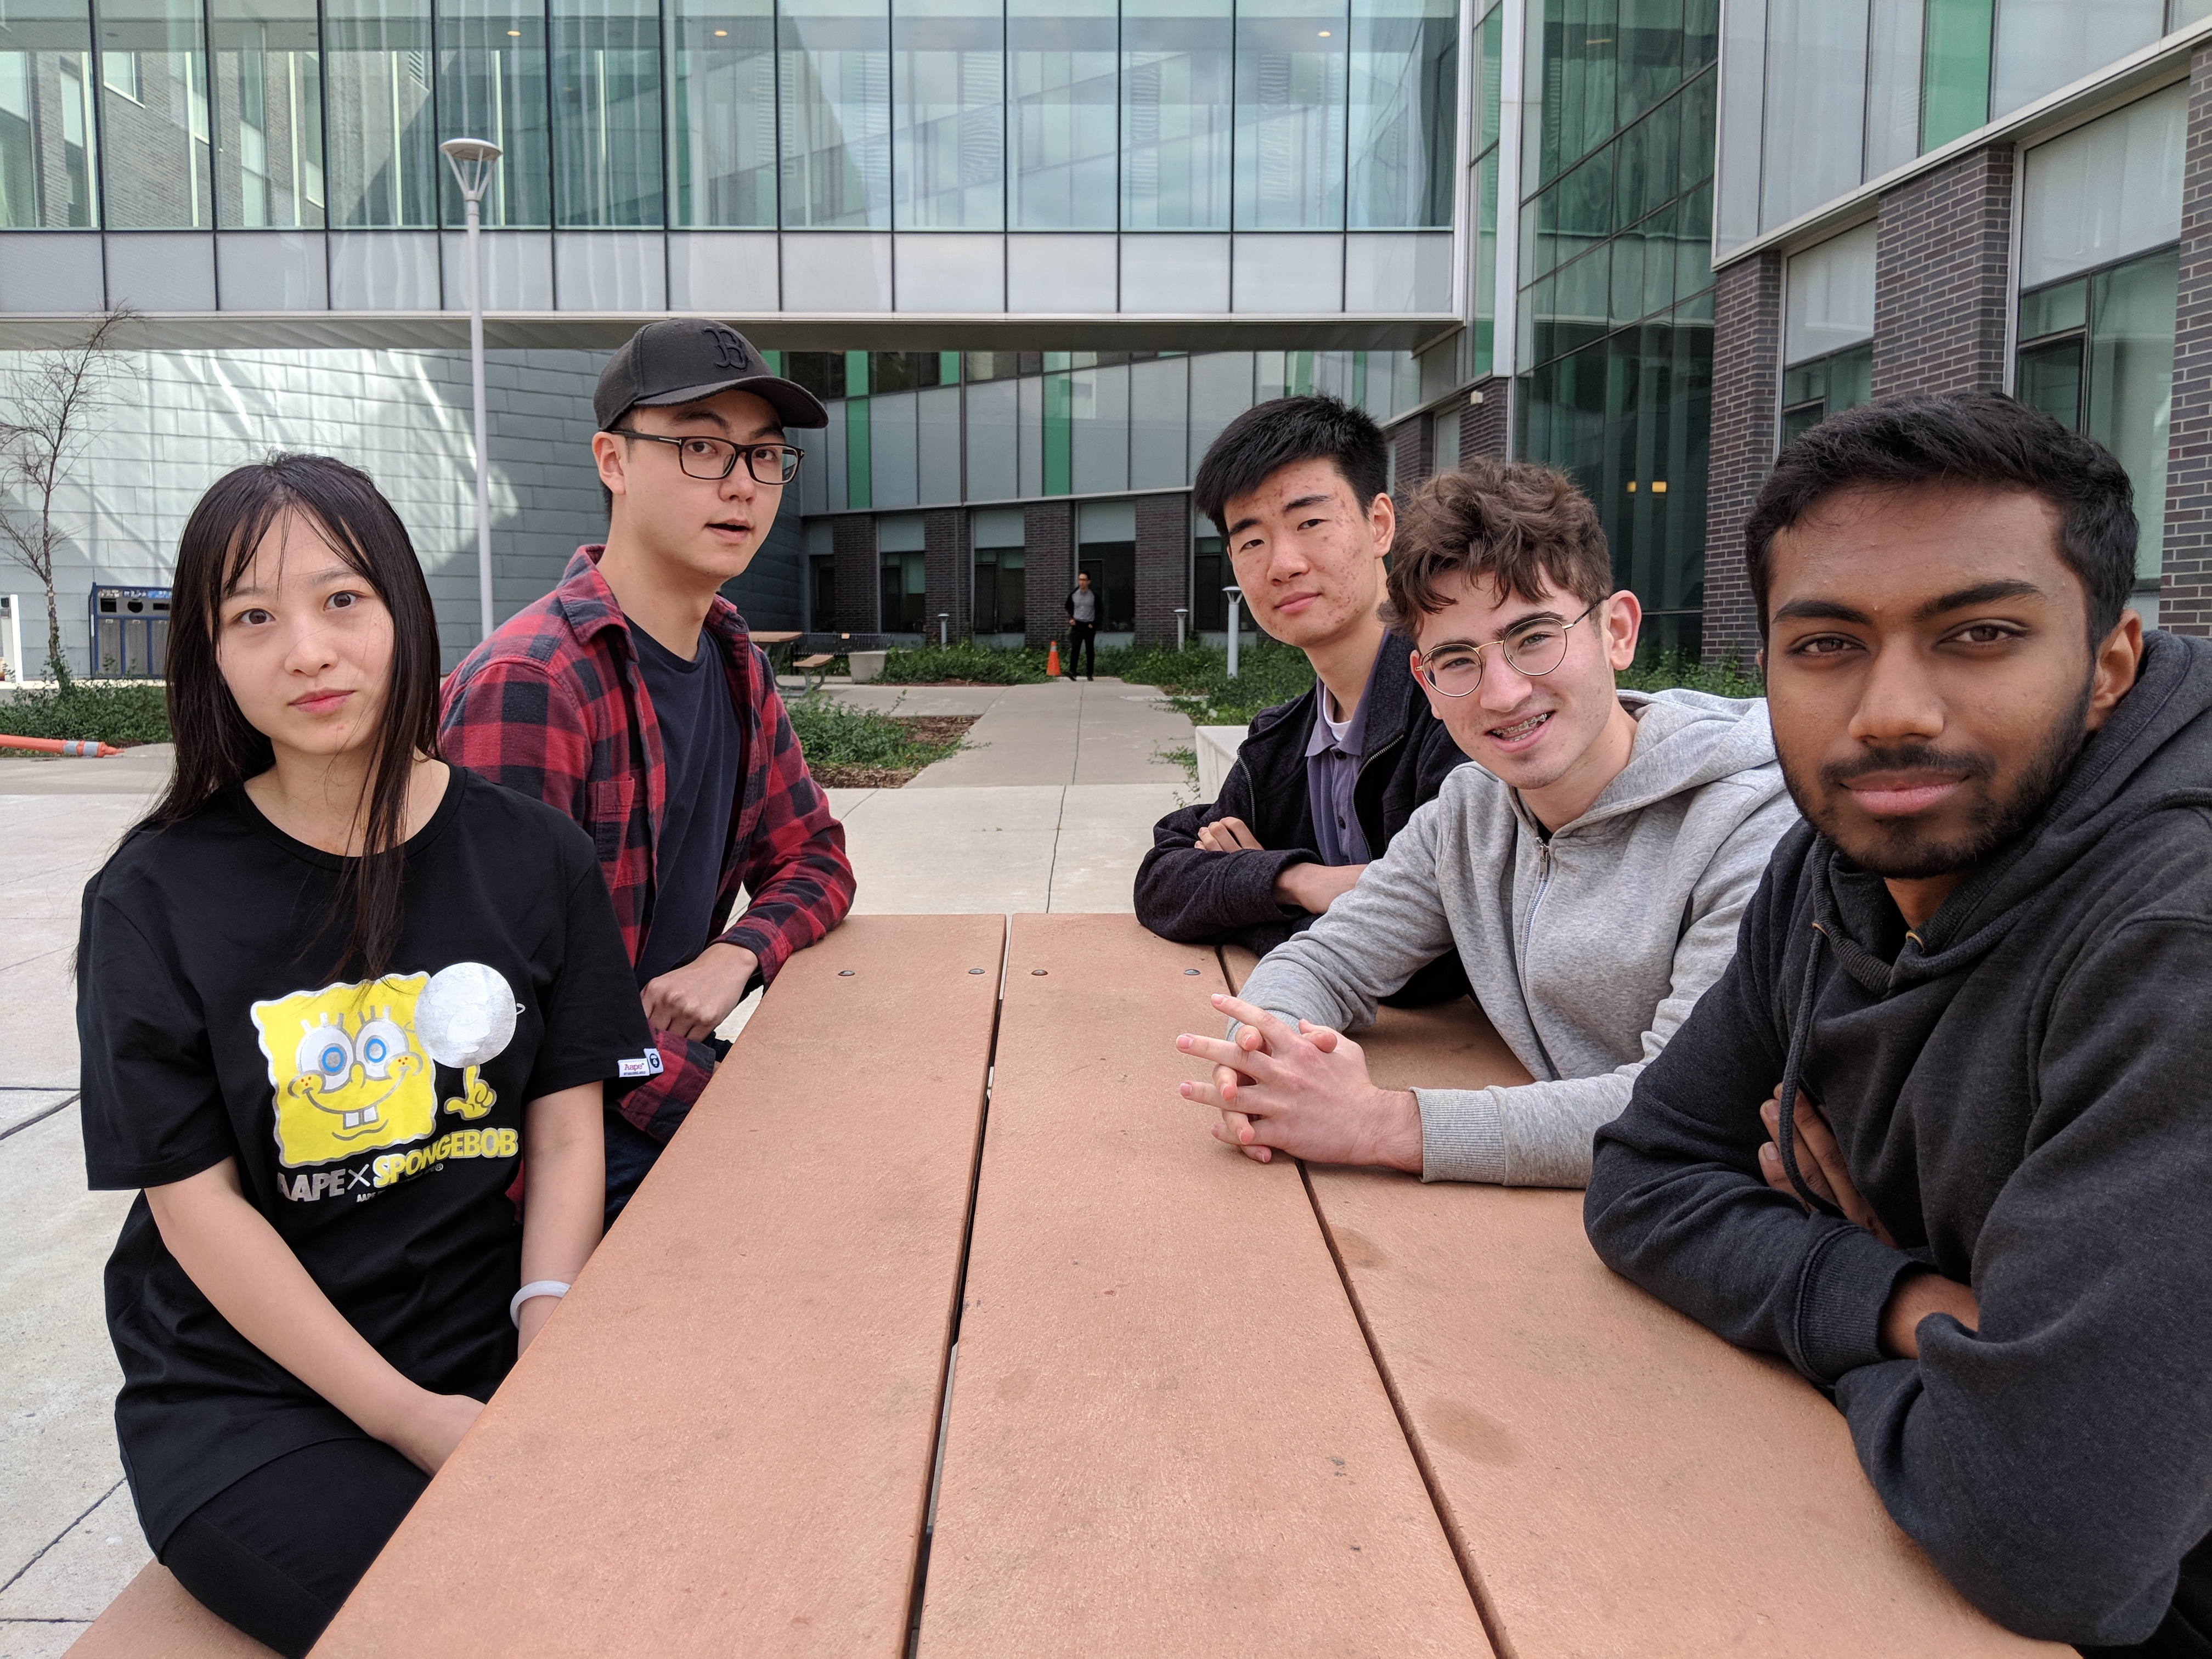
\includegraphics[width=0.9\textwidth]{team.jpg}}
\captionof{figure}{Photo of the whole team}
\centering{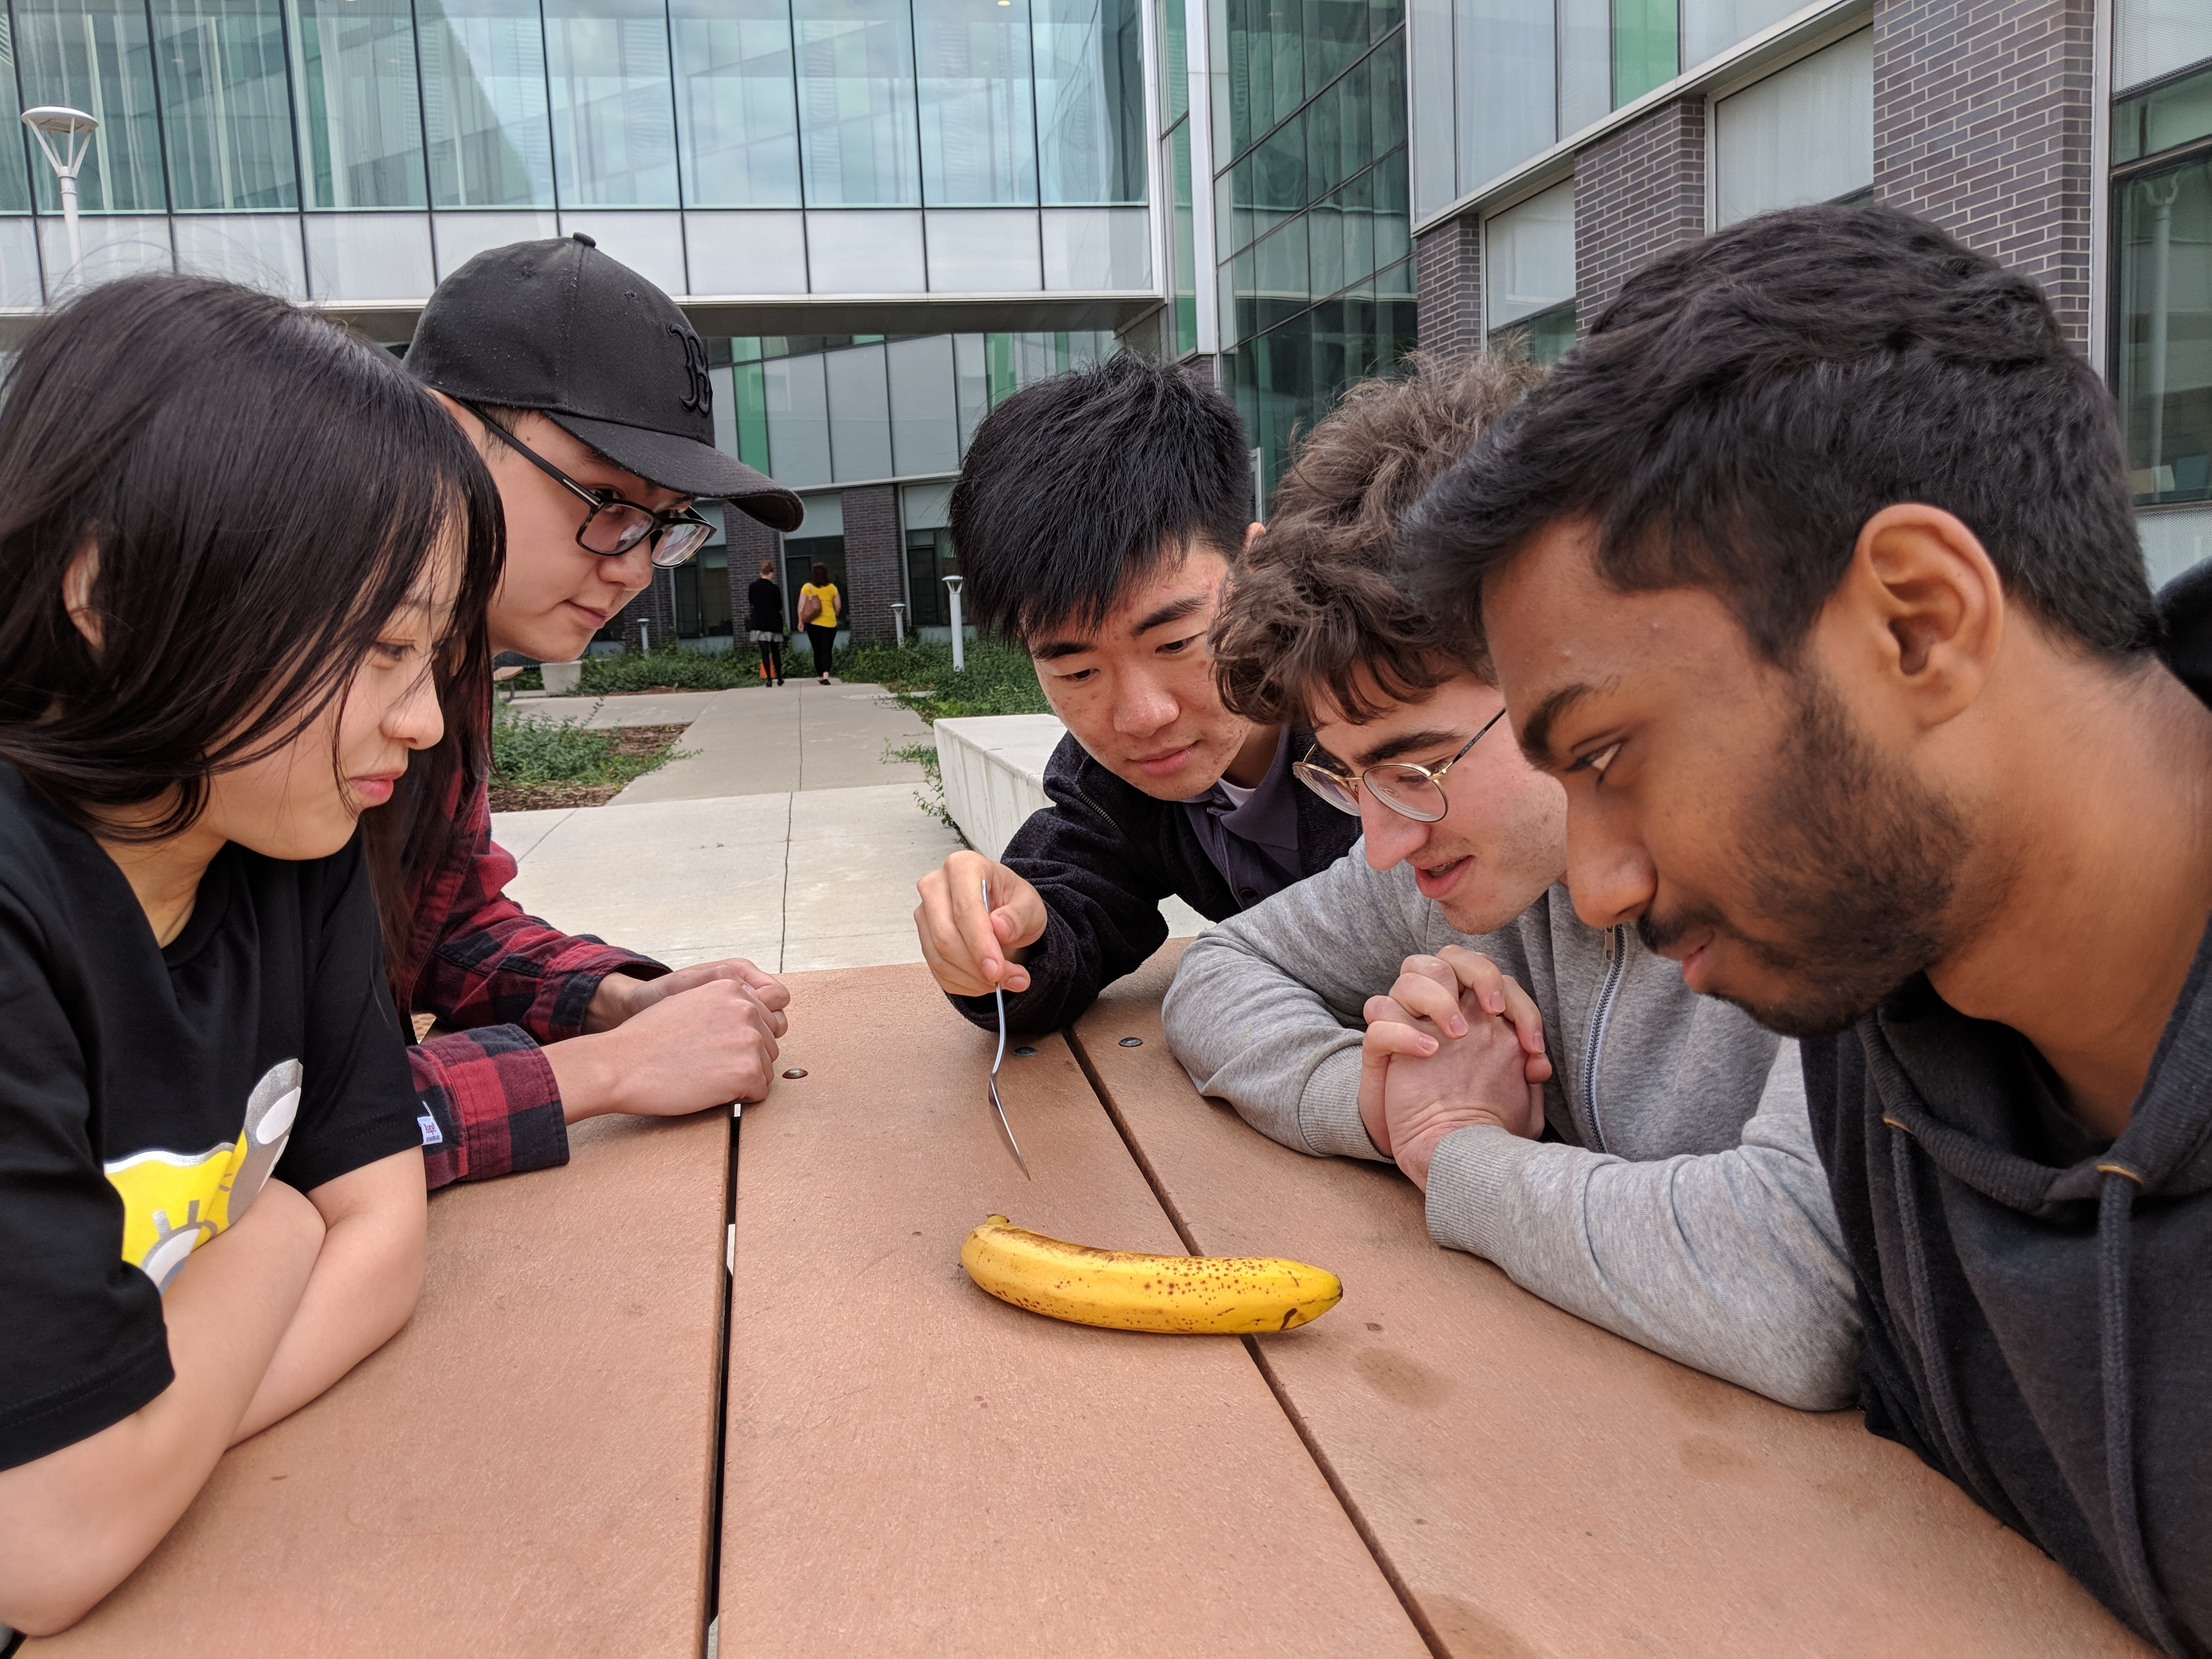
\includegraphics[width=0.8\textwidth]{food1.jpg}}
\captionof{figure}{Photo of team anticipating the consumption of a banana.}
\vspace{0.5cm}
\centering{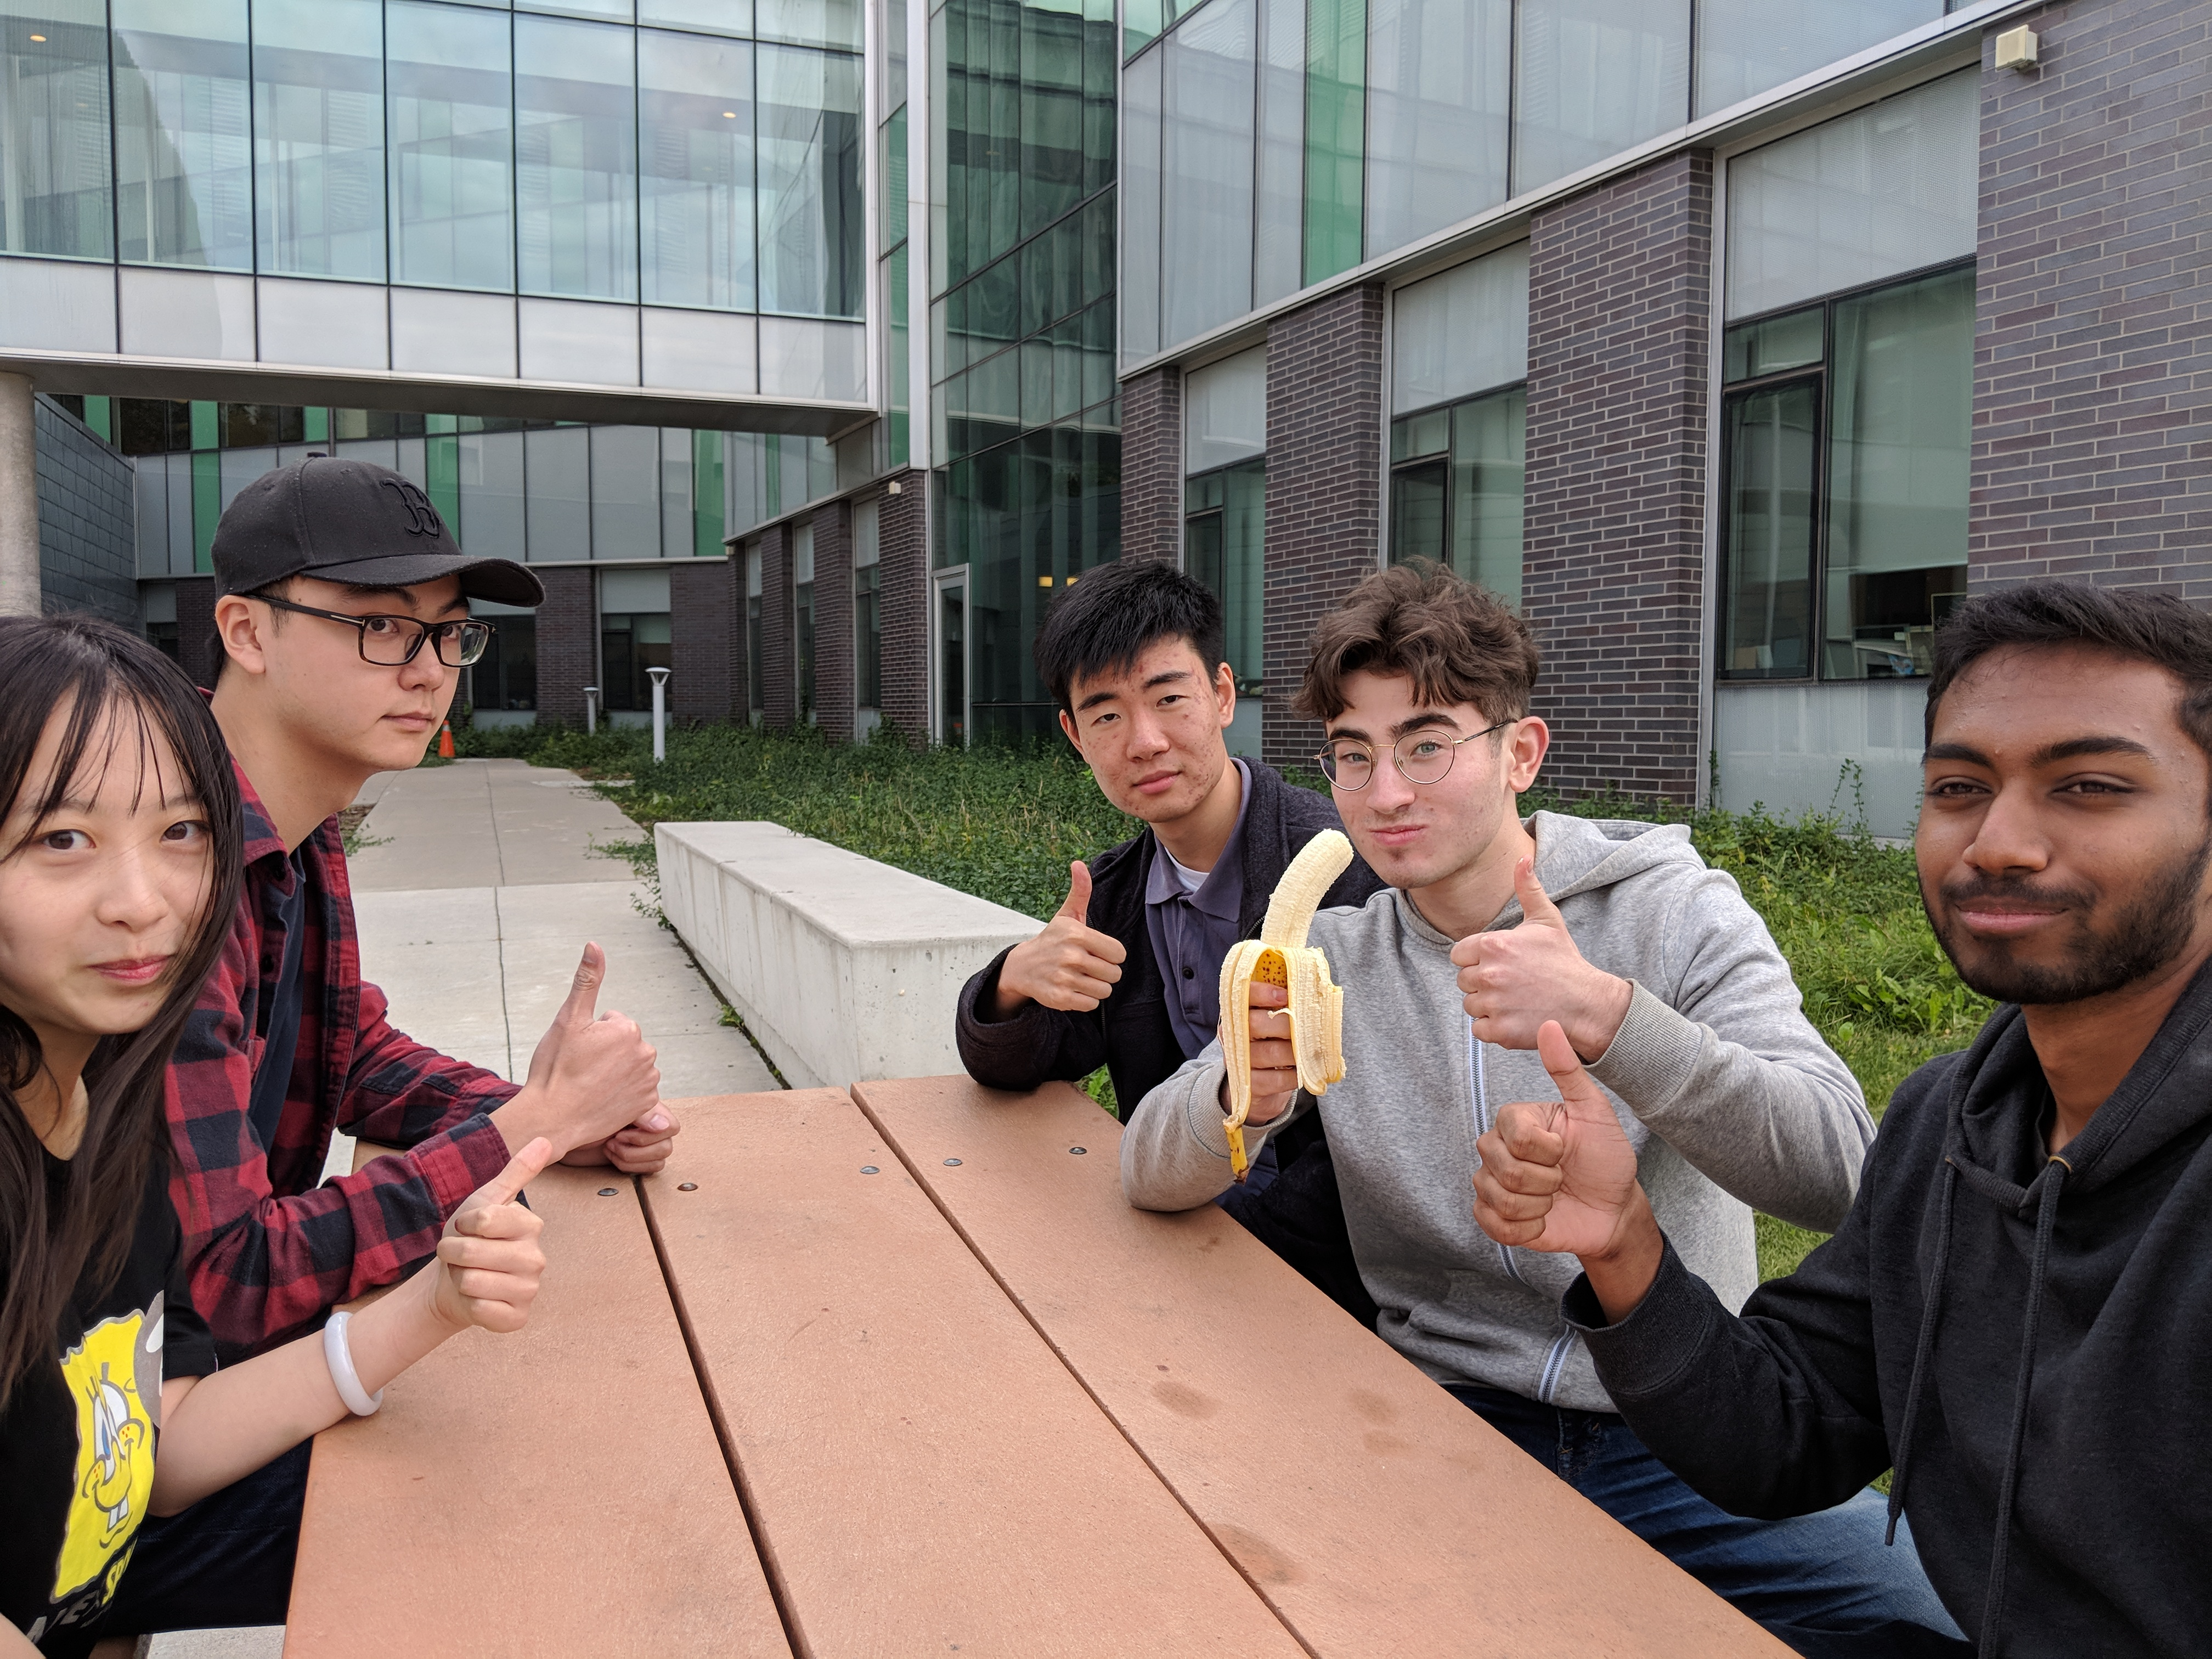
\includegraphics[width=0.8\textwidth]{food2.jpg}}
\captionof{figure}{Consumption of banana.}

\subsection{Our goals}
\begin{enumerate}
	\item Create a product that exceeds client expectations
	\item Use agile practices to be an efficient, productive and organised
	\item Improve existing skills and knowledge of software tools
	\item Learn new technologies and gain experience using them
	\item Establish good rapport with client to have more productive discussions of requirements
	\item Understand the needs of the client to create features they didn't even know they wanted
\end{enumerate}

\end{document}          
